%! suppress = MissingLabel
\documentclass[11pt]{article}

% Packages
\usepackage{amsmath}
\usepackage{float}
\usepackage{graphicx}
\usepackage{sidenotes}
\usepackage[a4paper,
innermargin=2cm,
textwidth=12cm,
marginparwidth=5cm,
marginparsep=1cm,
heightrounded,
]{geometry}
\usepackage{etoolbox}
\usepackage{setspace}
\AtBeginEnvironment{quote}{\singlespacing\small}

\let\oldemph\emph
\renewcommand{\emph}[1]{\oldemph{\textbf{#1}}\marginpar{\textbf{#1}}}


%% Draw line
\usepackage{tikzpagenodes}

\usepackage{atbegshi}
\usepackage{csquotes}

\def\drawcode{%
\tikz [remember picture, overlay] \draw
([xshift=.5cm]current page text area.north east)
--
([xshift=.5cm]current page text area.south east);}

\AtBeginDocument{% For the first page
\drawcode}

\AtBeginShipout{% For the remaining pages
\drawcode}

% Document
\begin{document}
    \section{Introduction}

    \emph{Gartner Hype Cycle}:
    \begin{itemize}
        \item \emph{Innovation trigger} future, commercial value unknown
        \item \emph{Peak of inflated expection} specific success stories with a lot of restrictions
        \item \emph{Through of Disillusionment} understanding of limitations of technology
        \item \emph{Slope of Enlightment} use understanding to develop commercially viable usage
        \item \emph{Plateau of Productivity} technology becomes mainstream
    \end{itemize}

    \begin{figure}[H]
        \centering
        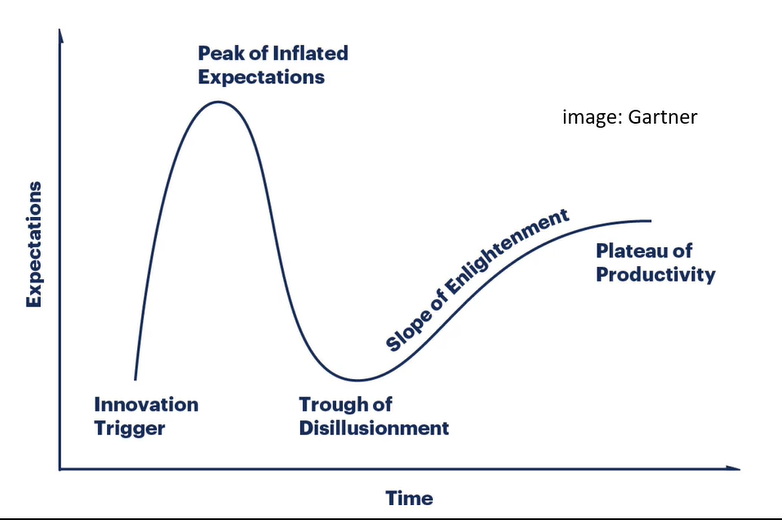
\includegraphics[width=0.8\textwidth]{img/hype.png}
        \caption{Hype}
        \label{fig:hype}
    \end{figure}

    \begin{figure}[H]
        \centering
        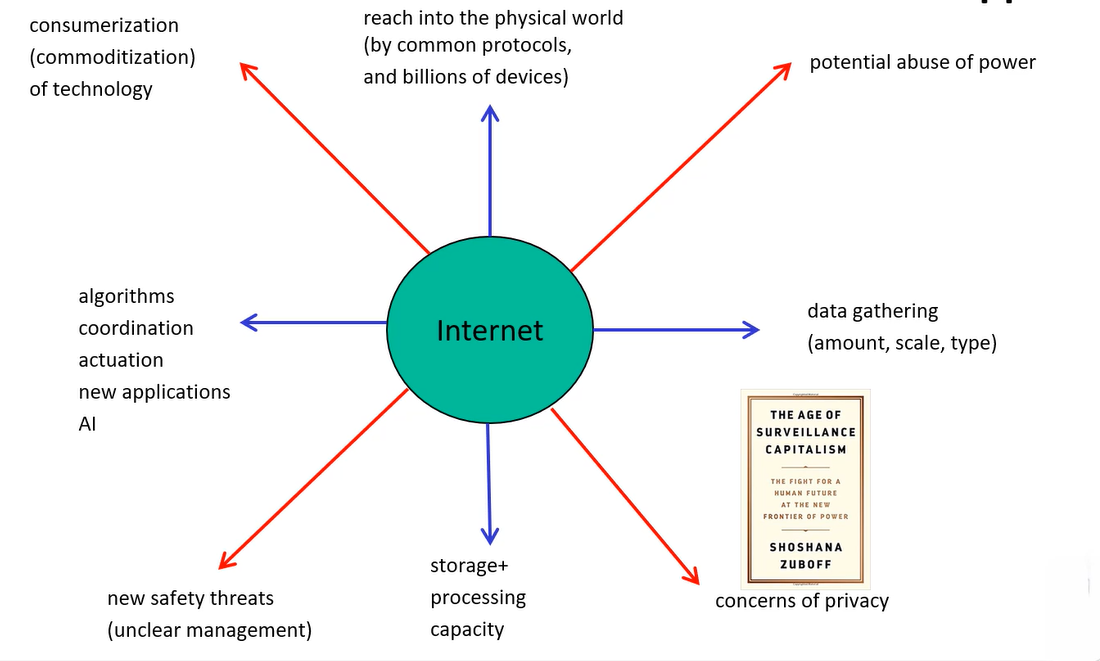
\includegraphics[width=0.8\textwidth]{img/internet.png}
        \caption{Internet}
        \label{fig:internet}
    \end{figure}

    Mainly focus on blue arrows in Fig~\ref{fig:internet}.

    \section{Examples}

    \subsection{Monitoring Energy Use example}

    \paragraph{Schematic}
    \begin{itemize}
        \item Red: direct data
        \item Red dotted: indirect data
        \item Blue: direct control
        \item Blue dotted: indirect control
    \end{itemize}

    \paragraph{Transformer}
    Report transformer data.
    \paragraph{Raspberry Pi}
    Create and provide overview report.
    Store data from smart meter.
    \paragraph{Smart meter}
    Report metering data.

    \paragraph{Questions}
    Which management concerns, where do we find management functionality, which quality concerns, who owns the data,
    what interests are there in the data, who controls the data, what are the `things'?

    \paragraph{3 tier architecture}
    UI, application, database.
    Many websites work like this.

    Architecture alternatives are obtained by different deployment choices of storing components on client machine and server machine.

    \paragraph{Integration}
    The system is composed of subsystems.
    Integration is at the network level.

    \paragraph{Data}
    \emph{Vertical analytics}:
    Data can be used to analyze processes in a home.

    \emph{Horizontal analytics}:
    Multiple homes can be monitored to learn about general things such as energy use, possibly using classification.

    \subsection{Quantified self}
    For proper horizontal analytics, not only monitor sick people, but also healthy people.

    \emph{Short cycle}:
    a standalone system that utilizes only the data of the individual.

    \begin{figure}[H]
        \centering
        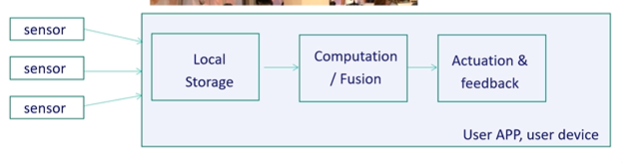
\includegraphics[width=0.8\textwidth]{img/short-cycle.png}
        \caption{Short cycle}
        \label{fig:sc}
    \end{figure}

    \emph{Long cycle}:
    employs a global storage of many users data, and horizontal analysis on that data.

    \begin{figure}[H]
        \centering
        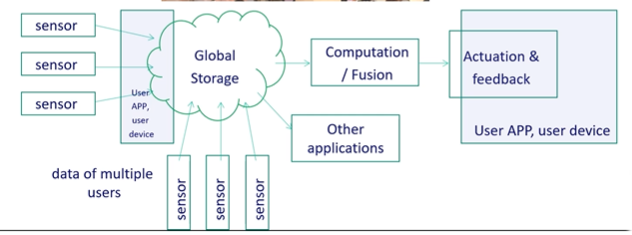
\includegraphics[width=0.8\textwidth]{img/long-cycle.png}
        \caption{Long cycle}
        \label{fig:lc}
    \end{figure}

    \emph{Alignment of platform owner and user}:
    user's interest is a personal outcome, and control over her own data.
    Platfor owner wants as much data as possible, obtain deep insight and market dominance.

    \section{Overview}

    \subsection{Definitions}

    Oxford \emph{IoT definition}:
    \begin{quote}
        Is the interconnection via the Internet of computing devices embedded in everyday objects, enabling them to send and receive data.
    \end{quote}

    Variety of definitions available, due to differences in scope (see p.3 of slides).
    We say: IoT = identifiable devices (attached to objects) and interconnected networks.

    \emph{Similar to internet}, but the IoT consists of devices
    \begin{itemize}
        \item with limited functions
        \item connected to low capacity networks
        \item without proper UI
        \item in large numbers (not just one-to-one)
        \item that interact with the real world
    \end{itemize}

    \paragraph{Scope}

    \begin{figure}[H]
        \centering
        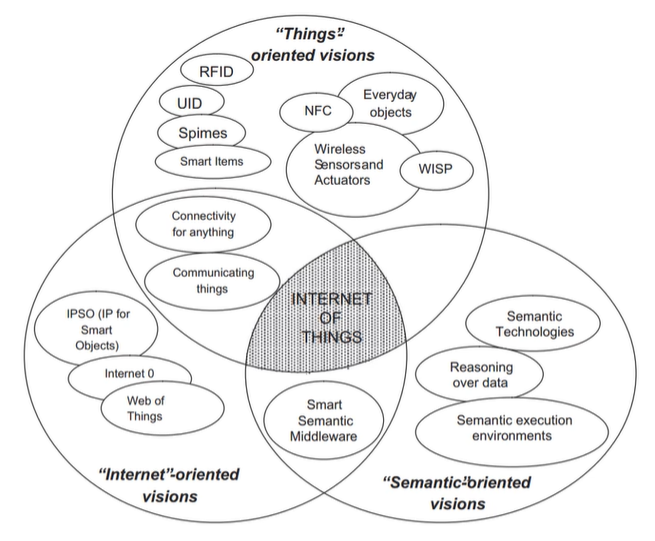
\includegraphics[width=0.8\textwidth]{img/paste-20201111123232.png}
    \end{figure}

    \emph{Cyber physical systems}: tight integration of communication, computation, physical world.

    \emph{Cloud computing}: build powerful services and applications on top of massive amounts of data, collected through embedded devices.

    IoT system consists of:
    \begin{itemize}
        \item Constrained devices (memory, processing power, energy, accessibility)
        \item Constrained networks (bitrate, packet loss, asymmetric links, etc)
        \item \emph{Internet services}: deal with large amounts of data and support processing
    \end{itemize}

    \subsection{Understanding IoT systems}
    \begin{itemize}
        \item Domains
        \item Architecture
        \item Communication stack and protocols
        \item Lifecycles of devices, services, applications
    \end{itemize}

    \section{Life Cycles}
    What is the life cycle of IoT systems and components and impact of application domain?

    \emph{Life cycle}:
    \begin{quote}
        The life cycle of a product or system is the series of stages it goes through from inception to decline.
    \end{quote}

    Typical: analysis, design, implementation, testing, maintenance, repeat.
    Life cycles for IoT pertain to devices, services and applications.
    Because, IoT applications are networked, which means the system is distributed and deployment and commisioning are cumbersome.
    Life cycles differ per domain.
    Lice cycle stages have typical use cases, and are key to understanding IoT architectural requirements.

    \begin{figure}[H]
        \centering
        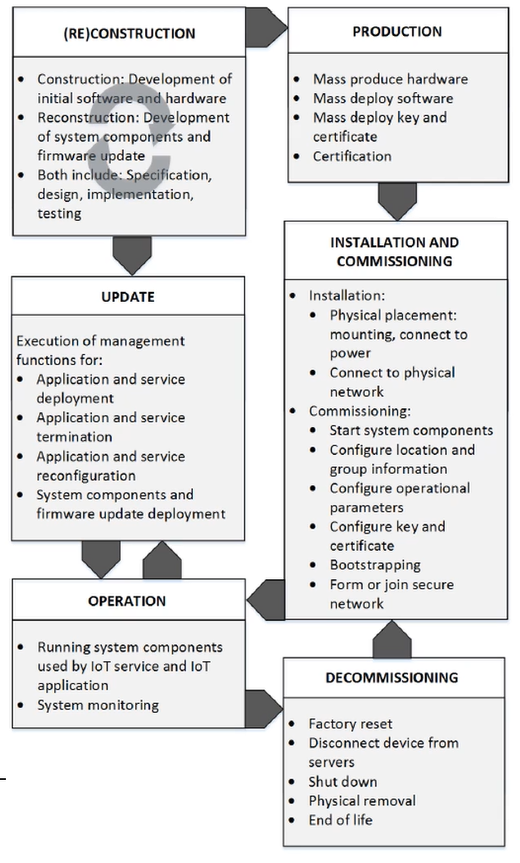
\includegraphics[width=0.8\textwidth]{img/paste-20201111124953.png}
        \caption{IoT device life cycle}
    \end{figure}

    Important: responsibilities and control of all stakeholders involved.

    Involved software types:
    \begin{itemize}
        \item Embedded operating system
        \item Libraries
        \item Components exposing services
        \item Applications
    \end{itemize}

    Software update packaging
    \begin{itemize}
        \item \emph{Firmware}: OS and middleware
        \item \emph{Module}: library/application
        \item \emph{Setting}: parameter setting
    \end{itemize}

    \begin{figure}[H]
        \centering
        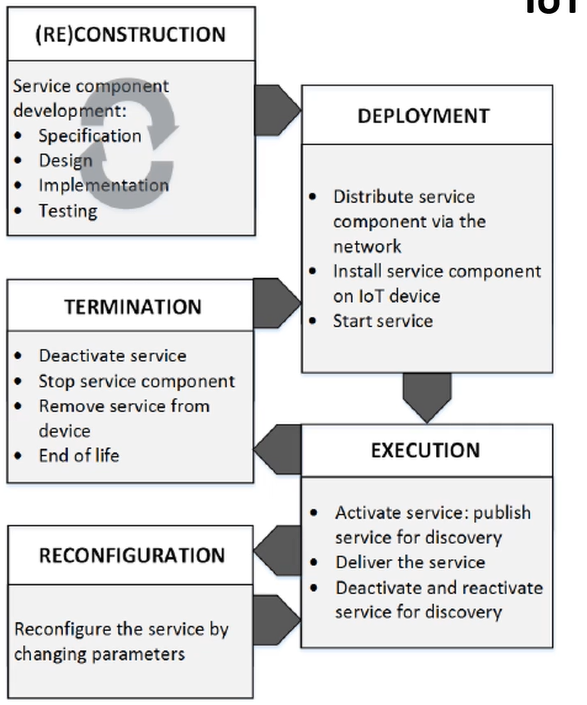
\includegraphics[width=0.8\textwidth]{img/paste-20201111125632.png}
        \caption{IoT service and component life cycle}
    \end{figure}

    \begin{figure}[H]
        \centering
        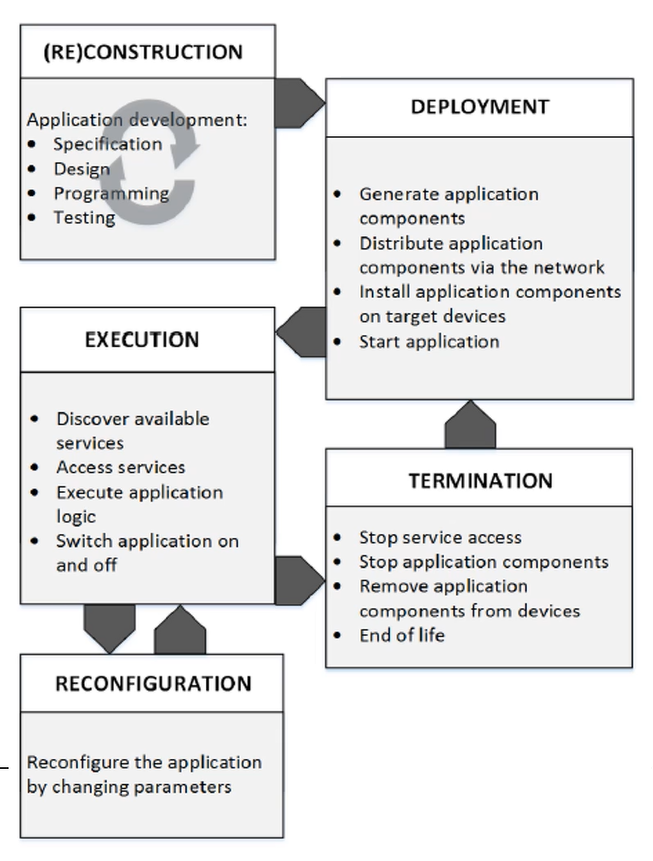
\includegraphics[width=0.8\textwidth]{img/paste-20201111125919.png}
        \caption{IoT application life cycle}
    \end{figure}

    Application life cycle depends on lice cycles of components and libraries (services).

    Extrafunctional properties:
    \begin{itemize}
        \item Security: trust new devices/components, access control, encryption, security management.
        \item Reliability, availability, safety: self monitoring
        \item Privacy: control on personal information
    \end{itemize}

    \paragraph{Characteristics of the home domain}
    The home is in principle unmanaged: one-time configuration, responsibility for software updates not assigned, problems/side effects very difficult to understand.

    \paragraph{Need for control function}
    Home needs more integration and brains: no gateway for everything, better network and equipment management, storage of history and persistent state, machine learning, etc.
    Use e.g.\ digital assistant (Google Assistant, Alexa, etc.)

    \paragraph{Characteristics of the office domain}
    The office is managed: central access control, clear procedures and responsibilities for system updates, standardization, higher cost acceptable.
    Conclicting concerns: bring your own device, data management.

    Other domains (city, industry) have further characteristics, have very implementation of lice cyles, and have different problems in life cycles.

    \section{Architecture}

    \subsection{Standards and platforms}
    Involved bodies and frameworks:
    \begin{itemize}
        \item ETSI (network)
        \item ITU (network)
        \item IETF (protocols)
        \item EU projects such as IoT-A, SENSEI for books and architectures
        \item OSG (data, information)
        \item OMA (Open mobile alliance)
        \item IEEE (protocols)
    \end{itemize}

    The war on standards,
    like Apple HomeKit, Google Home with Google Assistant, Microsoft with Azure IoT, Amazon with AWS IoT, Philips with HUE, etc.

    \subsection{Architecture}

    \begin{figure}[H]
        \centering
        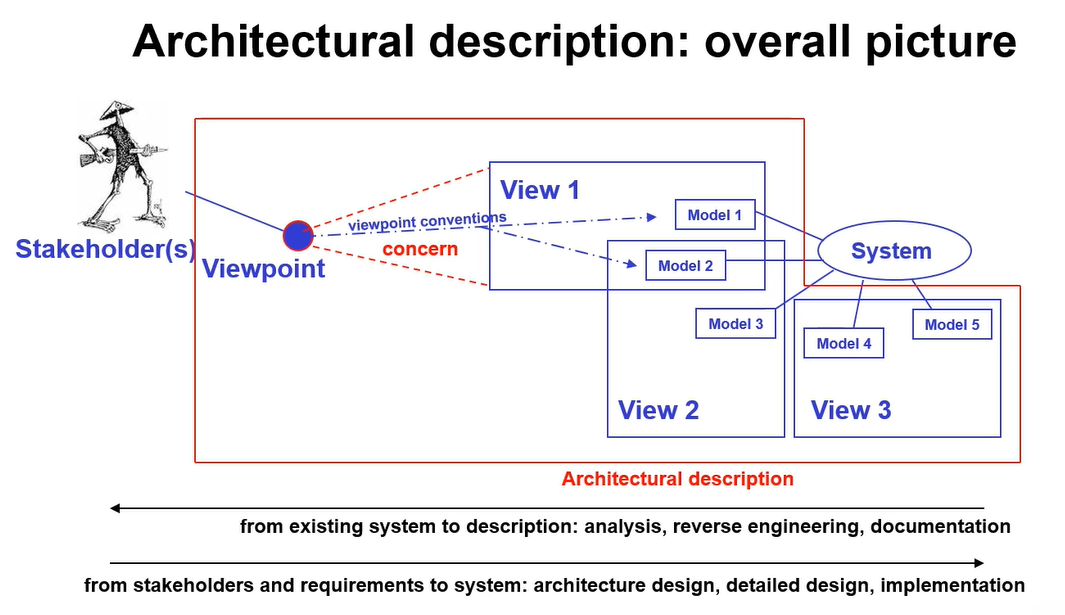
\includegraphics[width=0.8\textwidth]{img/paste-20201111132026.png}
        \caption{Architectural description}
    \end{figure}

    A collection of models organized into views that examine a system from a certain viewpoint defined by the concern of a stakeholder.
    For understanding, andalysis, communication, construction, documentation.

    \emph{Architecture definition}
    \begin{figure}[H]
        \centering
        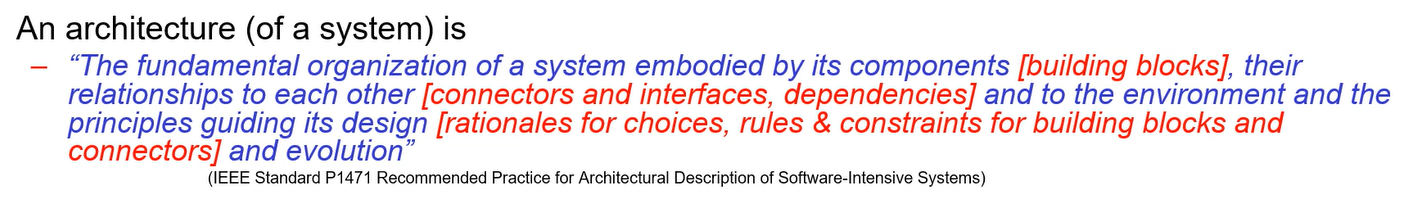
\includegraphics[width=0.8\textwidth]{img/paste-20201111132140.png}
        \caption{Architecture definition}
    \end{figure}

    Views and models:
    \begin{itemize}
        \item Logical layering/technical views: overall impression
        \item Deployment/physical view: organizational alternatives
        \item Development view: organization of software
        \item Process view: operation and interoperation, protocols, architectural patterns
        \item Data view: data semantics, protection, etc
    \end{itemize}

    \begin{figure}[H]
        \centering
        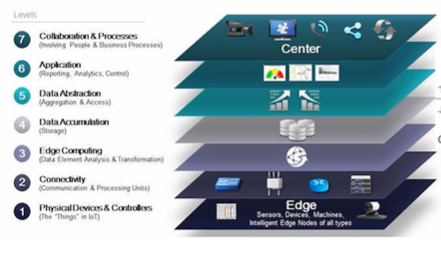
\includegraphics[width=0.8\textwidth]{img/stack.png}
        \caption{Reference model for IoT}
    \end{figure}

    \subsection{Deployment view}

    Physical elements
    \begin{itemize}
        \item `Things': Low capacity devices with sensors, actuators and an identifier
        \item Infra structure: switches, routers (connectivity with network technology), gateways (converting between parties, different layers of OsI stack), networks
        \item Storage devices
        \item User devices; phones, tablets, etc
        \item Embedded devices
        \item `Fog'; high capacity devices in the vicinity of data generation
        \item `Clouds': massive storage and execution power
    \end{itemize}

    Mapping IoT Arch. elements to devices, balance the following:
    \begin{itemize}
        \item Functional: sensing, actuating, application logic, communication, storage, data information, management
        \item Extra functional: dependability, performance, QoS, resource management, interoperability, mobility, ownership
        \item Boundary conditions: distributed systems, given components and protocols, network standards, legal matters
    \end{itemize}
    Think about \emph{Reliability vs. availability} and \emph{Security vs. privacy}

    \paragraph{Analytics}
    \emph{Vertical analytics}: Data from single unit.
    \emph{Horizontal analytics}: Data from many units.

    \paragraph{Managerial domain}
    Extra-functional domain, control span of a managing stakeholder.
    \emph{Physical managerial domain}: defined by physical access to domain and networks.
    \emph{Logical managerial domain}: Control over software elements and data.
    Derived from physical domain.

    Types of managerial control:
    \emph{Life cycle control}: Control over actions in life cycle like switching on/off.
    \emph{Behavioral control}: Controlling the behavior of a device or software element when it `runs'.

    \paragraph{Architeture alternatives}
    Take into account life cycles of devices/services/applications, and requirements set by all stakeholders.

    \paragraph{Communication}
    \begin{itemize}
        \item \emph{Broker}: A component that handles and translates calls between two or more parties.
        \item \emph{Proxy}: A component that acts on behalf of another component, implementing the same interface, and sometimes caching.
        \item \emph{Store}: One component leaves data and another one picks it up.
    \end{itemize}

    \begin{itemize}
        \item \emph{Push}: Control flow and data go in same direction (`call-back', `event driven').
        \item \emph{Pull}: Control flow and data go in poosite direction (`call', `polling')
    \end{itemize}

    \paragraph{Privacy, safety and security}
    \begin{itemize}
        \item \emph{Privacy}: control over personal information.
        \item \emph{Safety}: Freedom from danger or risk on injury resulting from recognized but potentially hazardous events.
        \item \emph{Security}: Regulating access to assets according to some policy.
    \end{itemize}


\end{document}